\subsubsection{Equations}
% \frame{\tableofcontents[currentsubsection]}
\frame{\frametitle{Governing equations \citep{Spiegel1960}}
\begin{overprint}
\only<1>{
\begin{align}
	\rho_{0}\frac{D}{D{t}}{\mathbf{u}} =& -\nabla p + \left(-\alpha{T}+\beta\mu\right)\rho_{0}\mathbf{g} + \nu\rho_{0}\nabla^{2}\mathbf{u} \\
	\nabla\cdot\mathbf{u} =& 0 \\
	\frac{D}{D{t}}{T} + w\frac{d}{dz}T_{0} =& \kappa_T \nabla^{2}T \\
	\frac{D}{D{t}}{\mu} + w\frac{d}{dz}\mu_{0}=& \kappa_{\mu}\nabla^{2}\mu
\end{align}}
\only<2>{
\begin{align}
	\frac{1}{\rm{Pr}}\frac{D}{D{t}}{\mathbf{u}} =& -\nabla p + \left(-T+\mu\right)\mathbf{\hat{z}} + \nabla^{2}\mathbf{u},\rm{Pr}\equiv\frac{\nu}{\kappa_{T}} \\
	\nabla\cdot\mathbf{u} =& 0 \\
	\frac{D}{D{t}}{T} \pm w =& \nabla^{2}T \\
	\frac{D}{D{t}}{\mu} \pm \frac{w}{R_{0}}=& \tau\nabla^{2}\mu, R_{0}\equiv\frac{\alpha\left(T_{0z}-T_{\rm{ad},z}\right)}{\beta\mu_{0z}}, \tau\equiv\frac{\kappa_{\mu}}{\kappa_{T}}
\end{align}
The $+$ corresponds to FC and the $-$, ODDC.}
\end{overprint}
}

% \frame{\frametitle{Boundary conditions}
% \begin{columns}
% 	\column{125pt}
% 	\begin{itemize}
% 		\item Fixed outer vertical boundaries
% 		\item Periodic horizontal boundaries 
% 		\item Cross-element boundaries must be continuous and smooth
% 	\end{itemize}
% 	\column{175pt}
% 	\begin{figure}[h]
% 		\centering
% 			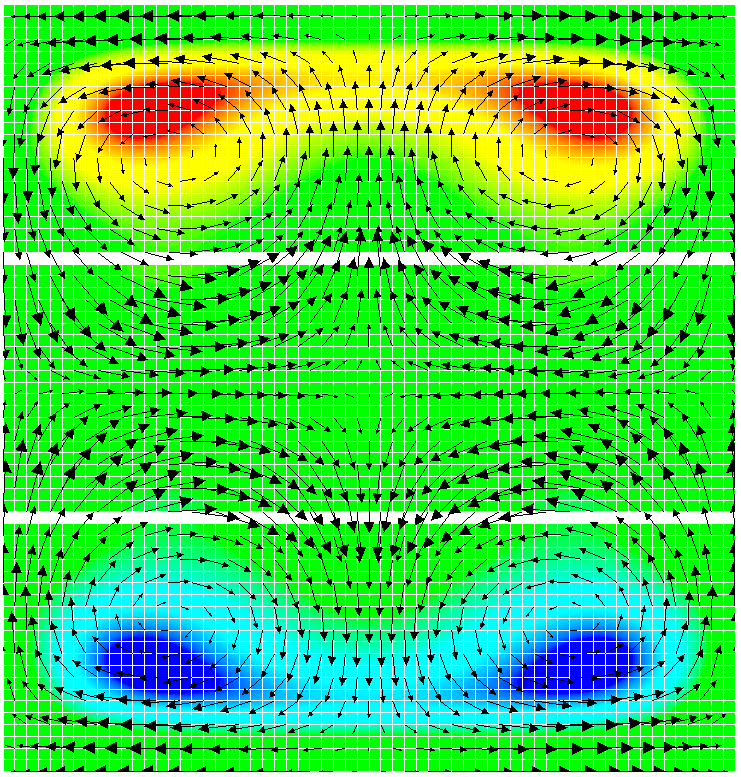
\includegraphics[width=0.8\textwidth]{figs/elements.png}
% 		\label{fig:figs_elements}
% 	\end{figure}
% \end{columns}}

\subsubsection{Spectral (Chebyshev)}

\frame{\frametitle{The code is pseudo-spectral, calculating the non-linear terms in Cartesian space and implicit terms in spectral space.}
\begin{overprint}
	\only<1>{
	\begin{itemize}
		\item Fourier series in the horizontal to enforce periodicity
		\item Chebyshev polynomials in the vertical for fine boundary resolution
	\end{itemize}
	\begin{equation}
		F\left(x,z\right)=\sum_{j=-N_{x}/2}^{N_{x}/2}\sum_{k=0}^{N_{z}}f_{i,j}e^{\frac{2\pi ij\left(x-x_{0}\right)}{L_{x}}}T_{k}\left(\frac{z-z_{0}}{L_{z}/2}\right) 
	\end{equation}
	}
\end{overprint}
}

\subsubsection{Dynamic Boundaries}

\frame{\frametitle{The extents of these elements are dynamic, and can be rezoned using simulated annealing.}
% \begin{overprint}
% 	\only<1>{
% We define $P (E (s), E (s'), T)$, the probability to accept a new state, $s'$, to maximize $E$, given a temperature, $T$, where $P > 0$ even if $E(s') < E(s)$ but that $P (E(s') < E(s)) \rightarrow 0$ as $T \rightarrow 0$.\footnote{Pseudocode from Wikipedia}
% \begin{itemize}
% 	\item Let $s = s_{0}$
% 	\item For $k$ in 0 to $k_{\rm{max}}$:
% 	\begin{itemize}
% 		\item $T =$ temperature ($\frac{k}{k_{\rm{max}}}$)
% 		\item Pick a random neighbor, $s'$ = neighbor ($s$)
% 		\item If $P(E(s), E(s'), T) >$ random(0, 1):
% 		\begin{itemize}
% 			\item $s = s_{\rm{new}}$
% 		\end{itemize}
% 	\end{itemize}
% 	\item Return: $s$
% \end{itemize}}
% \only<2>{
\begin{figure}
	\includemedia[width=\columnwidth,activate=onclick]{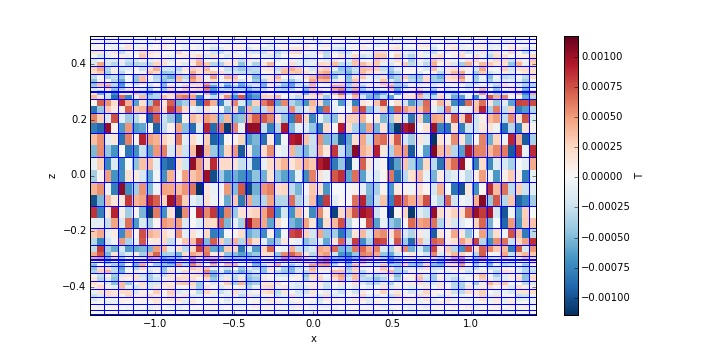
\includegraphics[width=\columnwidth,height=160pt]{out_00.png}}{out.swf}
\end{figure}
% }
% \end{overprint}
}